%%%%%%%%%%%%%%%%%%%%%%%%%%%%%%%%%%%%%%%%%
% Short Sectioned Assignment
% LaTeX Template
% Version 1.0 (5/5/12)
%
% This template has been downloaded from:
% http://www.LaTeXTemplates.com
%
% Original author:
% Frits Wenneker (http://www.howtotex.com)
%
% License:
% CC BY-NC-SA 3.0 (http://creativecommons.org/licenses/by-nc-sa/3.0/)
%
%%%%%%%%%%%%%%%%%%%%%%%%%%%%%%%%%%%%%%%%%

%----------------------------------------------------------------------------------------
%	PACKAGES AND OTHER DOCUMENT CONFIGURATIONS
%----------------------------------------------------------------------------------------

\documentclass[letterpaper, fontsize=11pt]{scrartcl} % A4 paper and 11pt font size

\usepackage[T1]{fontenc} % Use 8-bit encoding that has 256 glyphs
\usepackage{fourier} % Use the Adobe Utopia font for the document - comment this line to return to the LaTeX default
\usepackage[english]{babel} % English language/hyphenation
\usepackage{amsmath,amsfonts,amsthm} % Math packages

\usepackage{lipsum} % Used for inserting dummy 'Lorem ipsum' text into the template

\usepackage[]{mcode} %MATLAB code

\usepackage{sectsty} % Allows customizing section commands
\allsectionsfont{\centering \normalfont\scshape} % Make all sections centered, the default font and small caps

\usepackage{fancyhdr} % Custom headers and footers
\usepackage{graphicx}
\pagestyle{fancyplain} % Makes all pages in the document conform to the custom headers and footers
\pagenumbering{arabic}
\fancyhead{} % No page header - if you want one, create it in the same way as the footers below
\fancyfoot[L]{\textit{CME 102 Spring '15-'16}} % Empty left footer
\fancyfoot[C]{\thepage} % Empty center footer
\fancyfoot[R]{Tim Anderson} % Page numbering for right footer
\renewcommand{\headrulewidth}{0pt} % Remove header underlines
\renewcommand{\footrulewidth}{0pt} % Remove footer underlines
\setlength{\headheight}{13.6pt} % Customize the height of the header

\numberwithin{equation}{section} % Number equations within sections (i.e. 1.1, 1.2, 2.1, 2.2 instead of 1, 2, 3, 4)
\numberwithin{figure}{section} % Number figures within sections (i.e. 1.1, 1.2, 2.1, 2.2 instead of 1, 2, 3, 4)
\numberwithin{table}{section} % Number tables within sections (i.e. 1.1, 1.2, 2.1, 2.2 instead of 1, 2, 3, 4)

\setlength\parindent{0pt} % Removes all indentation from paragraphs - comment this line for an assignment with lots of text
\begin{document}

%----------------------------------------------------------------------------------------
%	TITLE SECTION
%----------------------------------------------------------------------------------------

\newcommand{\horrule}[1]{\rule{\linewidth}{#1}} % Create horizontal rule command with 1 argument of height

%----------------------------------------------------------------------------------------
%	PROBLEM 1
%----------------------------------------------------------------------------------------

\section*{Week 2 Section Problems}
\par Solve the following problems. If initial conditions are given, solve for all constants of integration. It is okay to leave answers in implicit form or with unsolved integrals. 

\begin{enumerate}
\item \textbf{Linearity:} Show that the following ODEs are linear. If they are nonlinear, identify the nonlinear term and show that this term is nonlinear.

\begin{enumerate}
\item $sin(x)y''' + y = e^x$
\item $y' + y^2 = tan(x)$
\item $y'' + 3sin(y) = 0$
\item $y' + y = e^x$ 
\item $y' + y = e^y$
\end{enumerate}

\item \textbf{Separation of Variables:} Solve the following using separation of variables. 
\begin{enumerate}
\item $y' = cot(y)$ 

\item $y' = y - y_0$


\item $y' = 1 + e^{x} + e^{y} + e^{x + y}$ 

\end{enumerate}

\item \textbf{Direction fields, phase space, and stability:} For an ODE of the form $y' = f(x,y)$ (where $x$ and $y$ can also be vectors), we can find the fixed points through one of two ways. 
\begin{enumerate}
\item One method it to look at the direction field in $x$-$y$ space to find the fixed points and determine their stability. For the following figure, find the fixed points based on the direction field, and give their stability. \par
\begin{center}
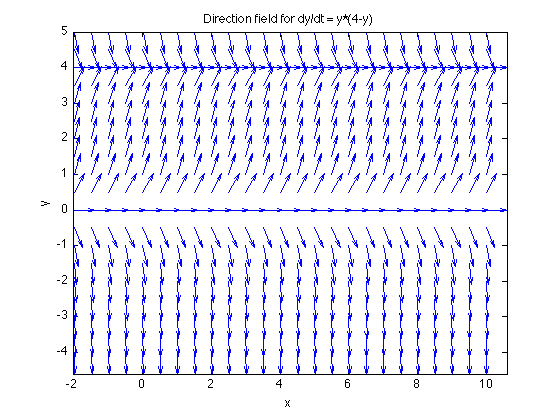
\includegraphics[width= 4in]{section2_1.png}
\end{center}
\item Another method is to examine function in what we call \textit{phase space}. This is where we plot the function value against its derivatives. In this case, we will plot the function in $y$-$y'$ space. For the following figure, find the fixed points by examine the function plotted against its derivative. Give the fixed points and their stability. \textit{Hint:} recall that a fixed point is where $y' = 0$. \newline
\begin{center}
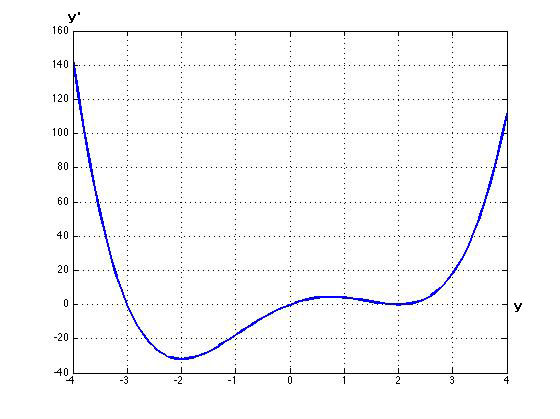
\includegraphics[width= 4in]{section2_2.jpg}
\end{center} 
\end{enumerate}


\item \textbf{MATLAB:} Write a \textit{small} piece of MATLAB code for each of the following functions. 
\begin{enumerate}
\item Output every multiple of 5 from 0 to 100. \textit{Hint:} the remainder of number $a$ after division by $b$ is given by mod($a$,$b$). 


\item Plot the functions $f_1(y) = y^2 + 1$ and $f_2(y) = y + 1$ over the domain $y \in [0,5]$ on the same graph in different colors with line thickness at 2pt. Pick a small enough increment in $y$ that the resolution of $f_1$ and $f_2$ is good. 

\item Write a function that will take two numbers as arguments and output their sum plus five i.e. $f(a,b) = a + b + 5$.  


\end{enumerate}

\end{enumerate}

%----------------------------------------------------------------------------------------

\end{document}